% Aspectratio 16:9 should be used
% The theme is not suited for 4:3 aspectratio
\documentclass[aspectratio=169]{beamer}

% Metadata of the presentation
\title{Technical analysis in bitcoin \\ \\ markets}
\date[ISBT 2018]{Internal Seminar - 12/02/2020}
\author[DB]{Niek Deprez --- \texttt{Niek.Deprez@UGent.be}}

% Load the UGent theme
\usetheme[language=en,faculty=eb,usecolors]{ugent}

% Have this if you'd like section slides 
\AtBeginSection[]{
    \sectionframe
}

\newcommand*{\captionsource}[2]{%
	\caption[{#1}]{%
		#1%
		\hspace{\linewidth}%
		{\footnotesize {\color{ugentblue}Source:} #2}%
	}%
}

\begin{document}

% Have this if you'd like the presentation to start 
% with a large UGent logo
%\logoframe

% I guess you always want a titleframe
%\titleframe

% Have this if you'd like a frame containing the 
% table of content
\begin{frame}{Overview}
    \tableofcontents[hideallsubsections]
    %Look at the current state of literature 
\end{frame}

\section{Introduction}

\begin{frame}
\frametitle{Motivation}
\begin{alertblock}{Is technical analysis profitable in bitcoin markets?}
	\begin{enumerate} 
		\item Why bitcoin?
		\item Why technical analysis?
	\end{enumerate}
\end{alertblock}
\end{frame}

\begin{frame}

\frametitle{Why bitcoin?}
\begin{block}{Bitcoin}
	\begin{itemize}
		\item Introduced in 2008 (Nakamoto, 2008)
		\item Electronic payment system based on cryptographic proof instead of trust
		\item No need for third parties
		\item instantaneous, low cost, anonymous worldwide payments
	\end{itemize}
\end{block}
\end{frame}

\begin{frame}
	\frametitle{Why bitcoin?}
	\begin{figure}
		\centering
		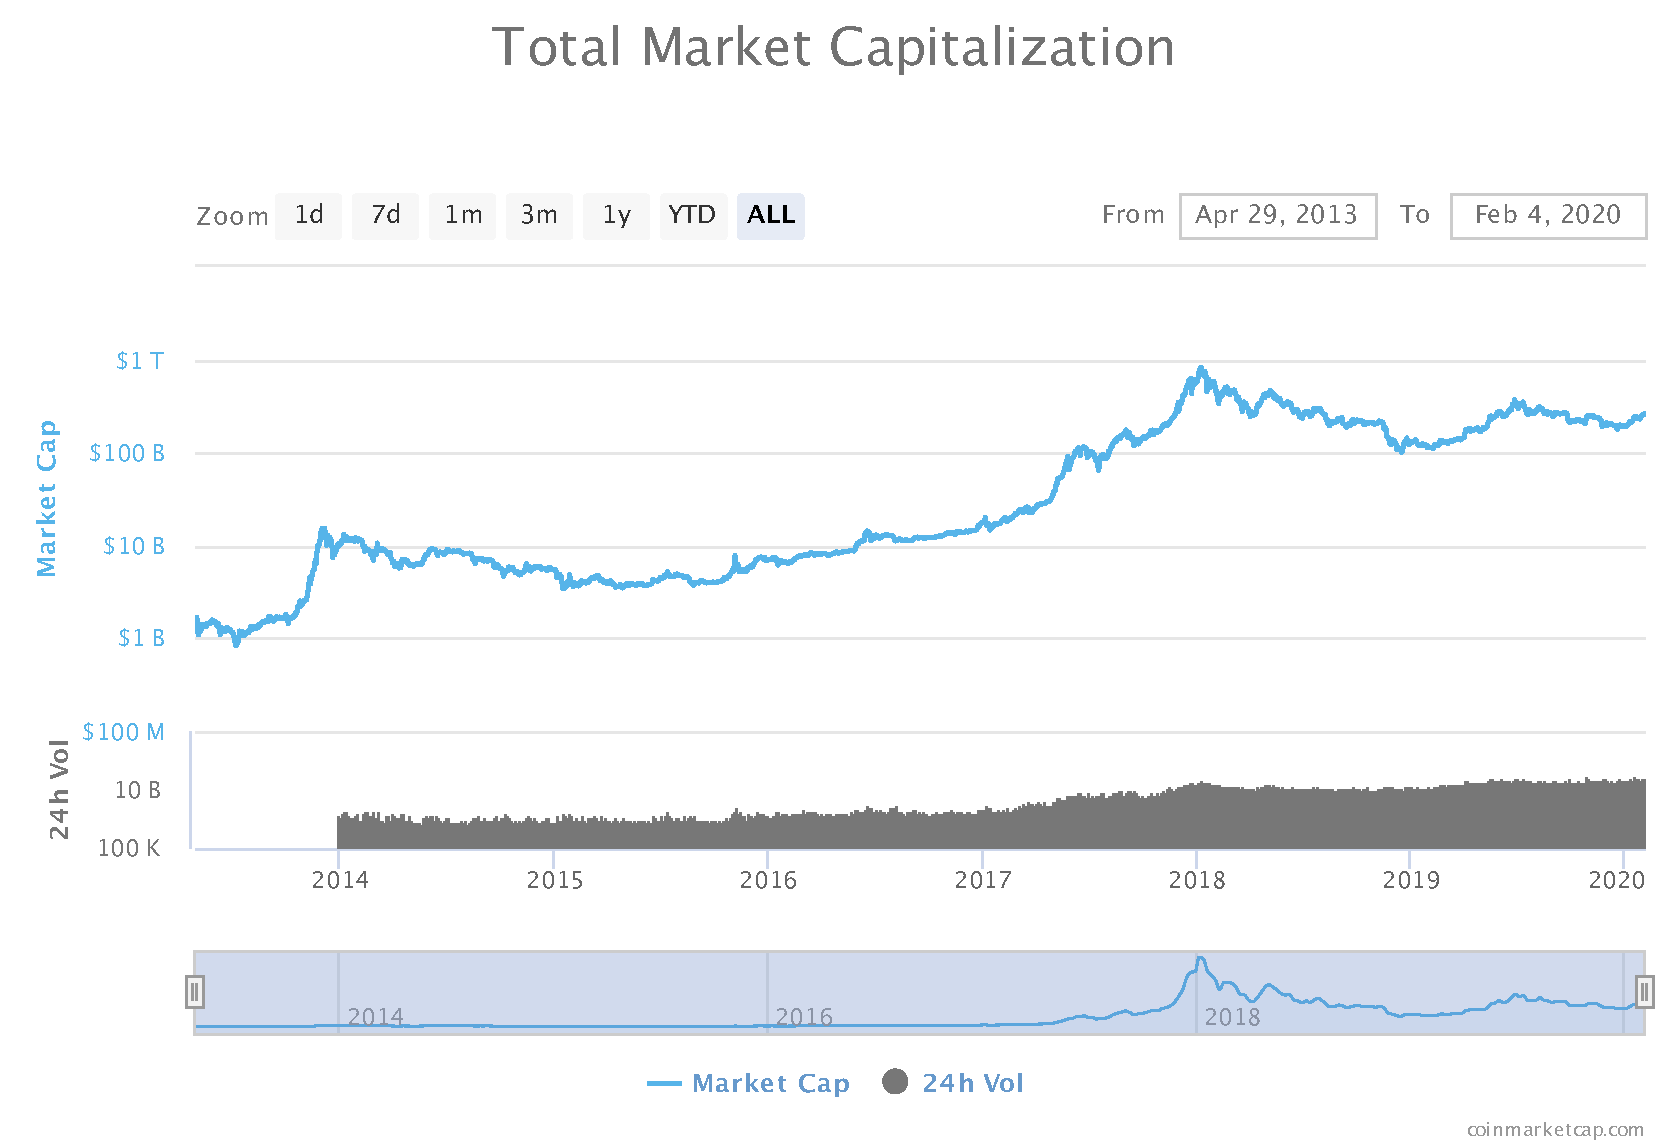
\includegraphics[width=0.8\linewidth, height=0.8\textheight]{total-market-capitalizat.pdf}
		\captionsource{Total market capitalization and 24h trade volume of the cryptocurrency market over time.}{https://coinmarketcap.com/charts/}
		\label{fig:marketcap}
		%Jan 14 10$B - 40$M
		%Jan 20 260$B - 110$B
	\end{figure}
\end{frame}

\begin{frame}
\frametitle{Why bitcoin?}
\begin{figure}
	\centering
	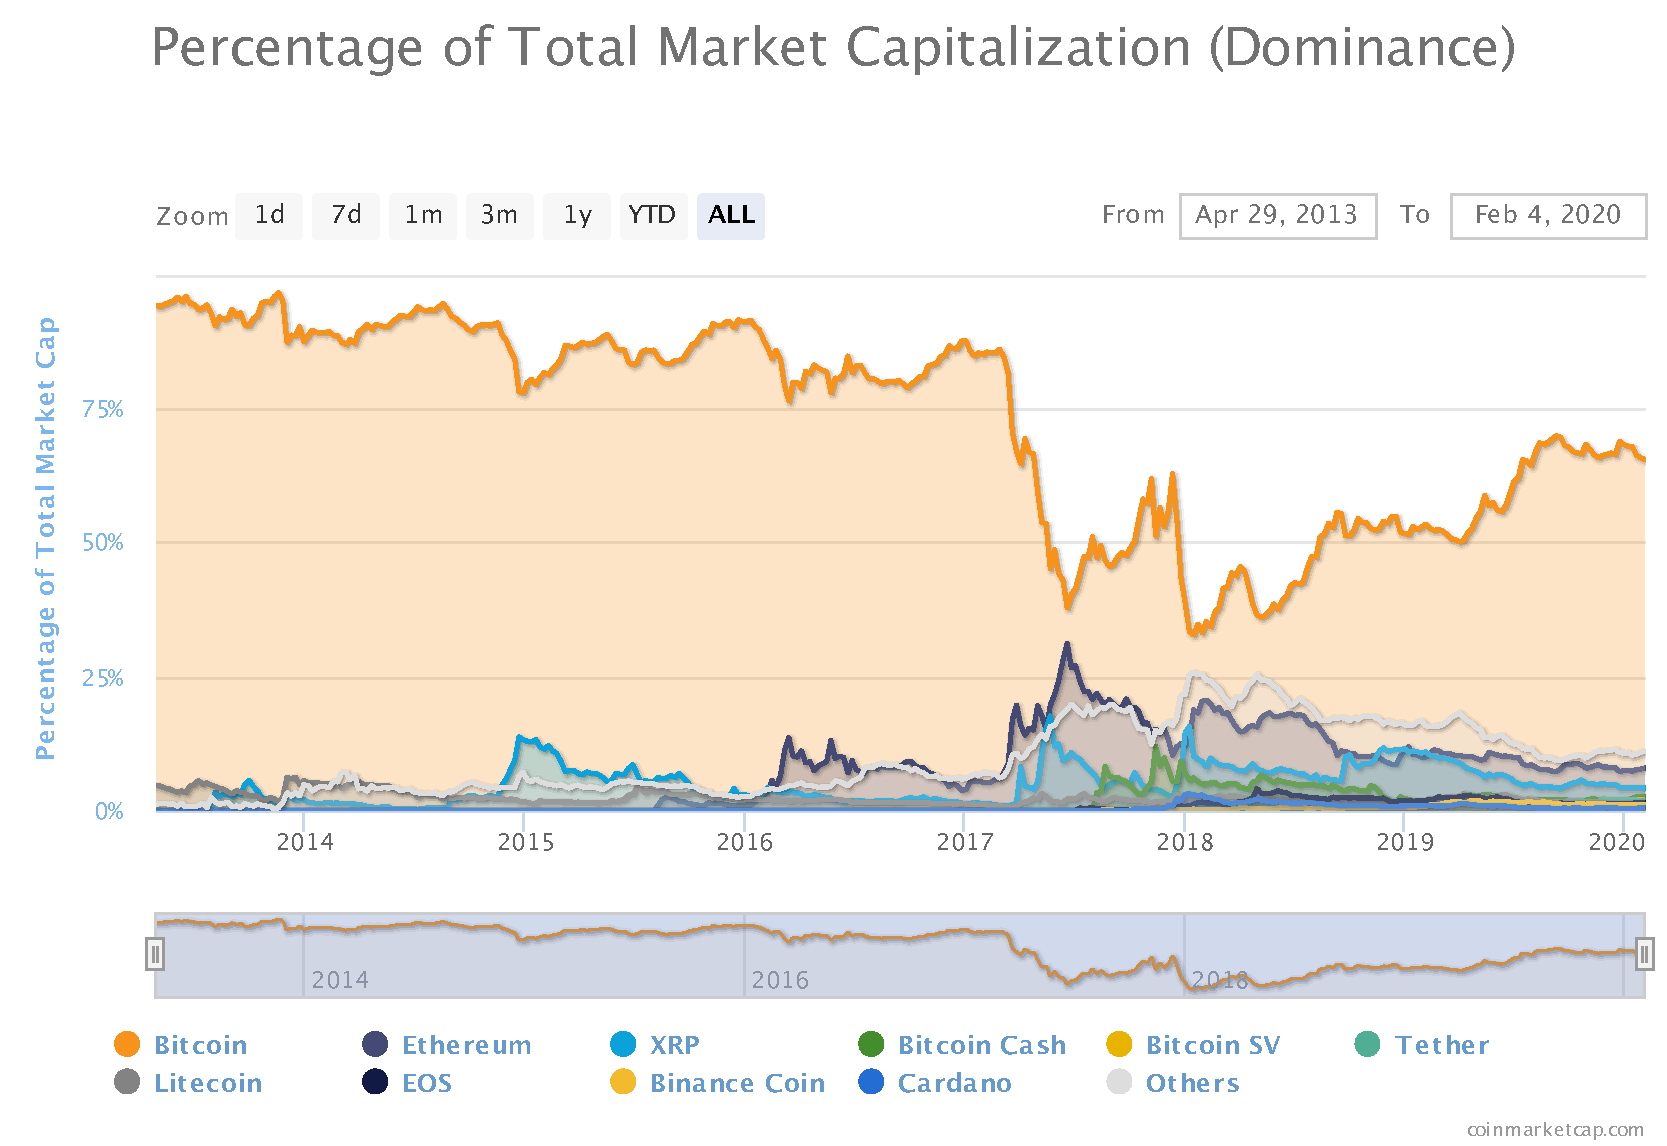
\includegraphics[width=0.8\linewidth, height=0.8\textheight]{percentage-of-total-mark.pdf}
	\captionsource{\% of total market capitalization of the cryptocurrency market over time.}{https://coinmarketcap.com/charts/}
	\label{fig:percmarkcap}
\end{figure}
\end{frame}

\begin{frame}
\frametitle{Why technical analysis?}
\begin{figure}
	\centering
	\includegraphics[width=0.9\linewidth, height=0.85\textheight]{../TechnicalAnalysisOnBitcoin1.1_files/figure-latex/exch_rate-1}
	\caption[Price of bitcoin over time.]{Price of bitcoin over time.}
	\label{fig:exchrate-1}
\end{figure}
\end{frame}


\begin{frame}
\frametitle{Why technical analysis?}
\begin{block}{Technical analysis}
	Using past prices in order to predict future returns. \\
	\begin{itemize}
		\item Requires inefficient markets
		\item Contested by academics, popular with professionals (especially FX)
	\end{itemize}
\end{block}



\end{frame}



\section{Methodology}
\section{Data}
\section{Results}

% Start of the first section
\section{Fonts and layout}

\begin{frame}
    \frametitle{This is the frame title}
    \framesubtitle{With optional frame subtitle}
    Regular text in the body of the slide is black and rendered in Helvetica sans-serif.\\[.5cm]
    Helvetica has no corresponding math font.
    Therefore, equations are typeset in Computer Modern sans-serif and are also displayed in plain black:
    \begin{equation*}
        F(x|\mu,s) = \int_{-\infty}^x s^{-1}\left(1+e^{-\frac{v-\mu}{s}}\right)^{-2} e^{-\frac{v-\mu}{s}}\;\mathsf{d}v = \frac{1}{1+e^{-\frac{x-\mu}{s}}}
    \end{equation*}
    Emphasis can be added by using \textbf{bold} typeface, \textit{italic}, {\color{ugent-alert}colors} or {\color{ugent-alert}\textbf{\textit{any combination}}}.\\
    More about colors follows later.
\end{frame}

\begin{frame}
    \frametitle{The frame title is rendered in Small Caps}
    The official UGent Powerpoint/Keynote templates have all titles in both ALL CAPS, \textbf{bold} and \underline{underline}.\\[.5cm]
    In my opinion, this combination is somewhat \underline{\textbf{AGGRESSIVE AND UNPLEASANT TO THE EYE}}.\\[.5cm]
    Instead, this theme makes use of \textsc{Small Caps} for all titles and subtitles
\end{frame}


\section{Lists and enumeration}

\begin{frame}
    \frametitle{Lists of items}
    This is how a list of unnumbered items looks:
    \begin{itemize}
        \item Item 1
        \item Item 2
        \item Item 3
    \end{itemize}
    \vspace{.25cm}
    Nested lists of items are possible too:
    \begin{itemize}
        \item Item 1
            \begin{itemize}
                \item Subitem a
                \item Subitem b
            \end{itemize}
        \item Item 2
            \begin{itemize}
                \item Subitem a
                \item Subitem b
            \end{itemize}
    \end{itemize}
\end{frame}

\begin{frame}
    \frametitle{Lists of items}
    This is how a list of numbered items looks:\\[.25cm]
    \begin{enumerate}
        \itemsep.5cm
        \item Item 1
        \item Item 2
        \item Item 3
        \item Item 4
        \item Item 5
    \end{enumerate}
\end{frame}


\section{Colors}

\begin{frame}
    \frametitle{Colors}
    \begin{itemize}
        \item The offical UGent colors (in RGB)  are part of the theme.
        \item The primary UGent color is {\color{ugentblue} ugentblue}, and the secondary color is {\color{ugentyellow} ugentyellow}.
        \item The faculty specific UGent themes can use the faculty color as secondary color.
            \begin{center}
                \begin{minipage}[t]{.35\textwidth}
                    \begin{itemize}
                        \item {\color{ugentblue}  \textbf{ugentblue}}
                        \item {\color{ugentyellow}\textbf{ugentyellow}}
                        \item {\color{ugent-lw}   \textbf{ugent-lw}}
                        \item {\color{ugent-re}   \textbf{ugent-re}}
                        \item {\color{ugent-we}   \textbf{ugent-we}}
                        \item {\color{ugent-ge}   \textbf{ugent-ge}}
                        \item {\color{ugent-ea}   \textbf{ugent-ea}}
                    \end{itemize}
                \end{minipage}%
                \begin{minipage}[t]{.35\textwidth}
                    \begin{itemize}
                        \item {\color{ugent-eb} \textbf{ugent-eb}}
                        \item {\color{ugent-di} \textbf{ugent-di}}
                        \item {\color{ugent-pp} \textbf{ugent-pp}}
                        \item {\color{ugent-bw} \textbf{ugent-bw}}
                        \item {\color{ugent-fw} \textbf{ugent-fw}}
                        \item {\color{ugent-ps} \textbf{ugent-ps}}
                    \end{itemize}
                \end{minipage}
                \vspace{.5cm}
            \end{center}
        \item Note that every faculty color name refers to the abbreviation of the faculty name.
    \end{itemize}
\end{frame}

\begin{frame}
    \frametitle{More about colors}
    \begin{itemize}
        \itemsep.25cm
        \item The main colors of the presentation are ugentblue, black and white.
        \item The secondary color should only be used exceptionally.
        \item The theme defines a special color \texttt{ugent-alert}.
        \item This color is \emph{or} {\color{ugentyellow}ugentyellow} \emph{or} the faculty color.
        \item The special color \texttt{ugent-alert} equals the faculty color:
            \begin{itemize}
                \item \textbf{if} the faculty specific template is used
                \item \textbf{and if} the option \texttt{usecolors} is set 
            \end{itemize}
        \item In all other cases \texttt{ugent-alert} is {\color{ugentyellow}ugentyellow}
    \end{itemize}
\end{frame}

\begin{frame}
    \frametitle{Example of ugent-alert}
    \begin{theorem}
        There is no largest prime number.
    \end{theorem} 
    \pause
    \begin{block}{Proof}
        \begin{enumerate} 
            \item<2-| alert@2> Suppose $p$ were the largest prime number. 
            \item<3-| alert@3> Let $q$ be the product of the first $p$ numbers. 
            \item<4-| alert@4> Then $q+1$ is not divisible by any of them. 
            \item<5-6| alert@5> But $q + 1$ is greater than $1$, thus divisible by some prime number not in the first $p$ numbers.\only<6>\qed
        \end{enumerate}
    \end{block}
\end{frame}

\begin{frame}
    \frametitle{Another example of ugent-alert}
    Blocks can be created for definition, proofs, examples, etc.
    \begin{block}{Regular block}
        This is an important message.
    \end{block}
    \vspace{.5cm}
    \pause
    A special kind of block is the \texttt{alertblock}:
    \begin{alertblock}{Alert!}
        This is a very important message.
    \end{alertblock}
\end{frame}


\section{Frame numbers}

\begin{frame}
    \frametitle{Frame numbers}
    \begin{itemize}
        \itemsep.25cm
        \item By default frame numbers are places on every ``regular'' frame.
        \item That excludes logoframes, titleframes and sectionframes.
        \item The frame number is always followed by the total number of frames.
        \item The theme option \texttt{noframenumber} removes frame numbers on all slides.
    \end{itemize}
\end{frame}

\section{Questions?}

% End presentation with titleframe
\titleframe

\end{document}
